\subsection{LetterLizardJS: JavaScript Letter Lizard Implementation}

% Introduce Language
% JAVASCRIPT
% - "language of the Web", implemented in Web browsers to allow client 
%   side scripts to interact with the user, control browser, preform 
%   asynchrous communication with server, alter docmuent that is displayed
% - also server-side programming, desktop and mobile applications
% - dynamic, prototype based
% - first class functions
% - syntax influenced by C, Java, but very different
% - key design principles takes from Self, Scheme
% - multi-paradigm: oop, imperative, functional
% - first introduced by Netscape, formalized as ECMAScript 
%
% - supports structured programming like C
% - exeption: function scoping instead of block scoping
% - many think that this was not a good idea (cite Definitive guide?)
% - automatic semicolon insertion (also not a good idea) (cite def guide?)
% - dynamic typing: types associated vith values, not variables
% - object based: objections are associative arrays with String or int
%   property names (special langauge support for arrays)
% - aside from a few primitive types, everything is an object, including
%   funcions (which means that funcitons are first-class enitiies - they
%   can be assigned to variables and even returned from other functions
% - event driven; 1st class funcs used a lot in event-driven browser/
%   run-time environment
% - closures (give an example or refer to later section)
% - objects augmented with prototypes; can be used to simulate "classical"
%   oop features
% - no distinction between func and method: caling convention

\pagebreak[4]
\global\pdfpageattr\expandafter{\the\pdfpageattr/Rotate 90}
\begin{sidewaysfigure}
	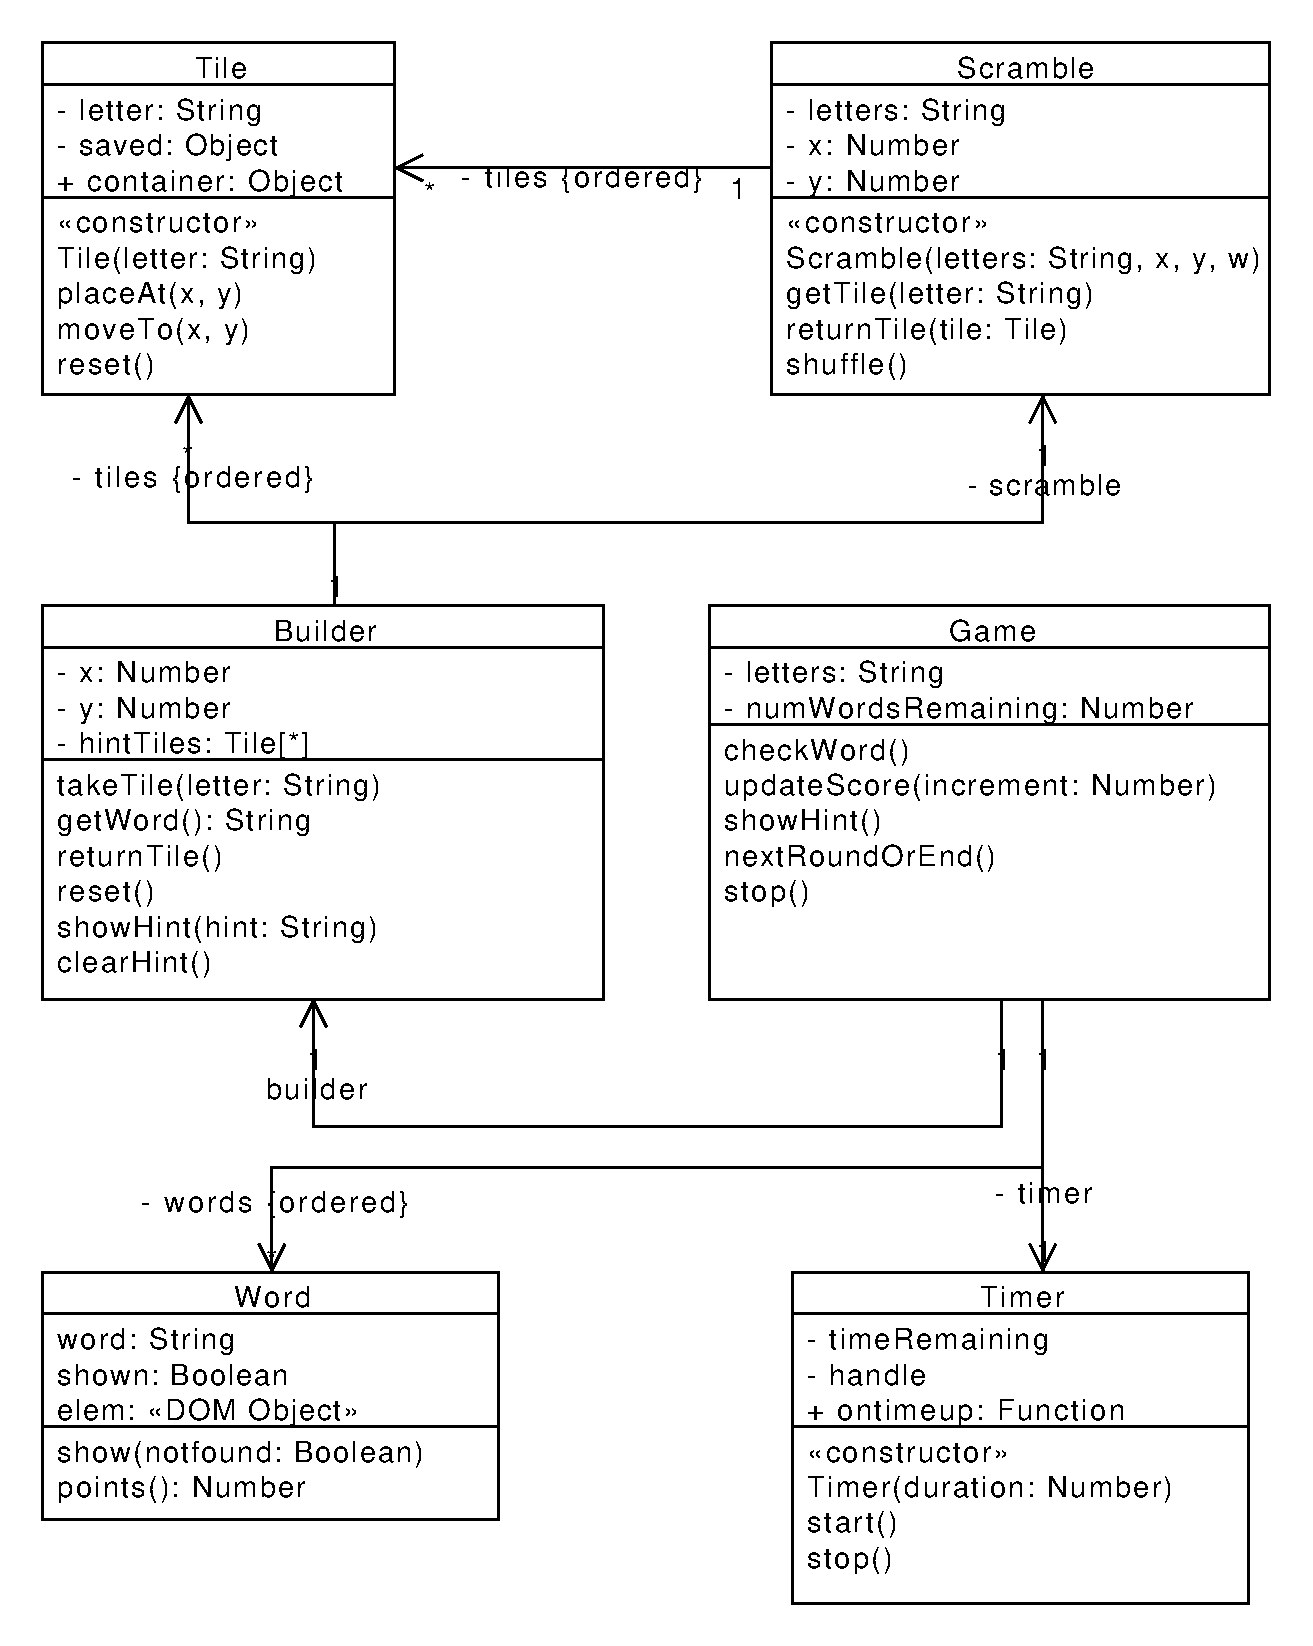
\includegraphics[scale=0.5]{../diagrams/LetterLizardJS-ClassDiagram.pdf}
\end{sidewaysfigure}

% talk about how this version is implemented (eg classes, etc)
% show screenshots
% talk about implementation: language features that were useful,
% class diagrams, sequence diagrams, snippets of code, etc